\section{Validity}\label{validity}

One of the primary goals of our software is to keep the user's sketch in
a valid state. Since our algorithms for plane detection and 3D
simulation succeed work if the edges form valid shapes, it is essential
to prevent invalid features from being added to the sketch. Therefore,
each feature has a function with the following signature, that validates
edges in a feature:

\begin{pygmented}{swift}
func validate() -> (passed: Bool, error: String) 
\end{pygmented}

The tool/template-based system is the primary means of insuring that
user input is valid. The validate function is a secondary system, which
attempts to fix errors in user input, and then returns an error message
if the feature could not be validated. In case of errors, the feature is
removed from the feature and we display a message using the warning
system. For example, the validate() method of v-fold features reads as
follows:

\singlespacing 

\begin{pygmented}{swift}
override func validate() -> (passed: Bool, error: String) {
 let validity = super.validate()    
 if(!validity.passed){
    return validity
 }
 // clever test for concave paths: close the vertical cut's
 // path and test whether vfold end point is inside it
 var testPath = UIBezierPath(CGPath: verticalCut.path.CGPath)
 testPath.closePath()
 if(testPath.containsPoint(diagonalFolds[0].end)){
    return (false,"Angle too shallow")
 }
 if(!tooShortEdges().filter({
    \$0.kind == Edge.Kind.Fold
    }).isEmpty){
        return (false,"Edges too short")
 }
    return (true,"")
 }
\end{pygmented}

\doublespacing

Here, we first validate using the superclass, performing checks that
apply to all features. Then, we perform checks specific to v-fold
features. V-folds are invalid if their form a convex polygon. To test
for this, we construct a straight line between the start and end of the
vertical cut, and then test whether the intersection point with the
driving fold lies within the closed shape. This feature type is also
invalid if any of its folds are shorter than a minimum edge length.

\begin{figure}[htbp]
\centering
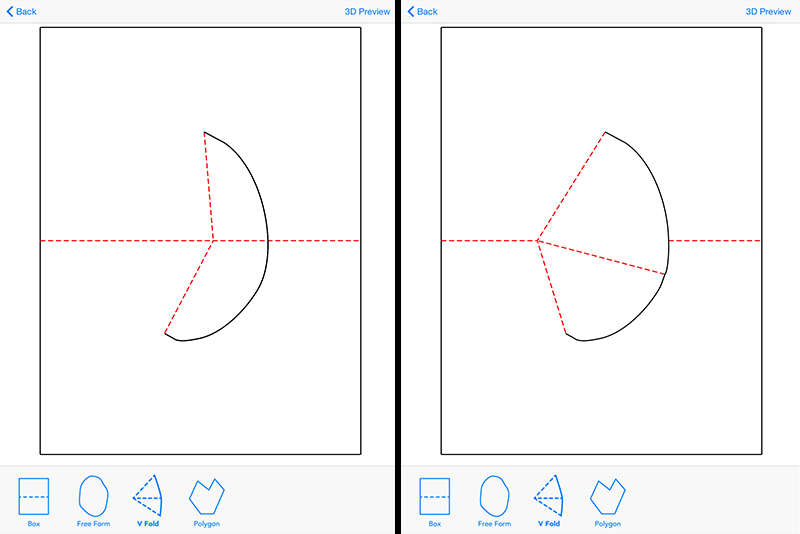
\includegraphics{figures/44_Tech_Validity/invalid_valid_vfold.png}
\caption{Left: an invalid, concave v-fold. Right: a valid, convex
v-fold.}
\end{figure}
